\section{Doxygen}
Zweck von Software Code Dokumentation ist die Wissensicherung, Kommunikation und das sichtbarmachen des Projektfortschrittes. Mittels Doxygen kann Code dokumentiert und ein entsprechends Dokument erzeugt werden. Damit findet man nicht Dokumentierte Parameter leichter und die Dokumentation bleibt konsistent mit Software. (WICHTIG: Doxygen ersetzt nicht Software-Dokumentation ansich!). 
\begin{center}
	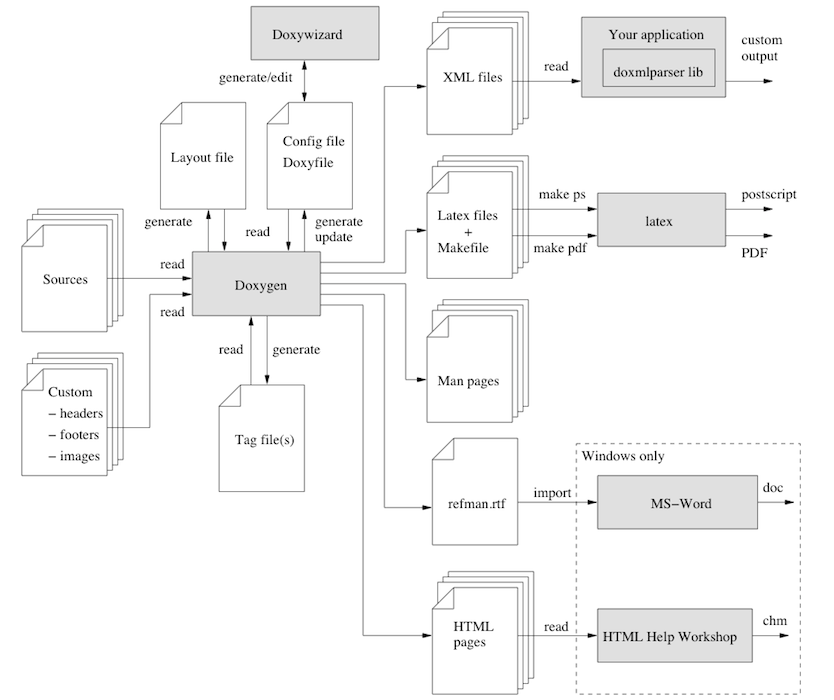
\includegraphics[width=\columnwidth]{Images/doxygen}
\end{center}

Die Wichtigsten Doxygen Funktionen (doxygen kann mittels \textit{doxygen.exe -g} eine neue Konfigurations Datei erstellen und mit  \textit{doxygen.exe ConfigFileName} gestartet werden):
\begin{itemize}[nosep]
	\item brief
	\item param
	\item pre*
	\item post*
	\item return
\end{itemize}
\begin{lstlisting}
///
/// \brief Calculates the optimal values for R1 and R2. The base formula
/// behind this calculation is \f$u1=u2 {r2 \over r2+r1}\f$.
/// \pre \p u1 > \p u2
/// \pre \p lowerRTh < \p upperRTh
/// \param u1 Value for U1 in V
/// \param u2 Value for U2 in V
/// \param lowerRTh set the lower bound for resistor value output
/// \param upperRTh set the higher bound for resistor value output
/// \param resDecade gives the resister e-decade on which the resistor are
/// calculated
///
virtual void calc(double u1, double u2, double lowerRTh, double upperRTh,
const EDecade& resDecade);
\end{lstlisting}